\documentclass{article}
\usepackage[T1]{fontenc}
\usepackage{lmodern}
\usepackage{graphicx}
\usepackage{amsmath,amssymb}
\usepackage[a4paper,margin=2cm]{geometry}
\usepackage[absolute,overlay]{textpos}
\setlength{\TPHorizModule}{1mm}
\setlength{\TPVertModule}{1mm}
\usepackage[indonesian]{babel}
\usepackage{hyperref}
\setlength{\emergencystretch}{2em}
% unit: Halaman 37

\begin{document}

% === Halaman 37 (llm) ===

\vspace{163.35mm}

\begin{itemize}
  \item Meskipun Eve dapat menyadap komunikasi antara Alice dan Bob, namun karena pesan sudah dienkripsi menjadi cipherteks, Eve tidak dapat memahami pesan yang disadapnya
\end{itemize}
\vspace{10mm}

% deskripsi: Diagram proses enkripsi dan dekripsi pesan antara Alice dan Bob dengan Eve sebagai penyadap yang hanya melihat cipherteks.
% bbox normalisasi: [0.1900, 0.3600, 0.7400, 0.9100]
\begin{textblock*}{115.50mm}(39.90mm,106.92mm)
\noindent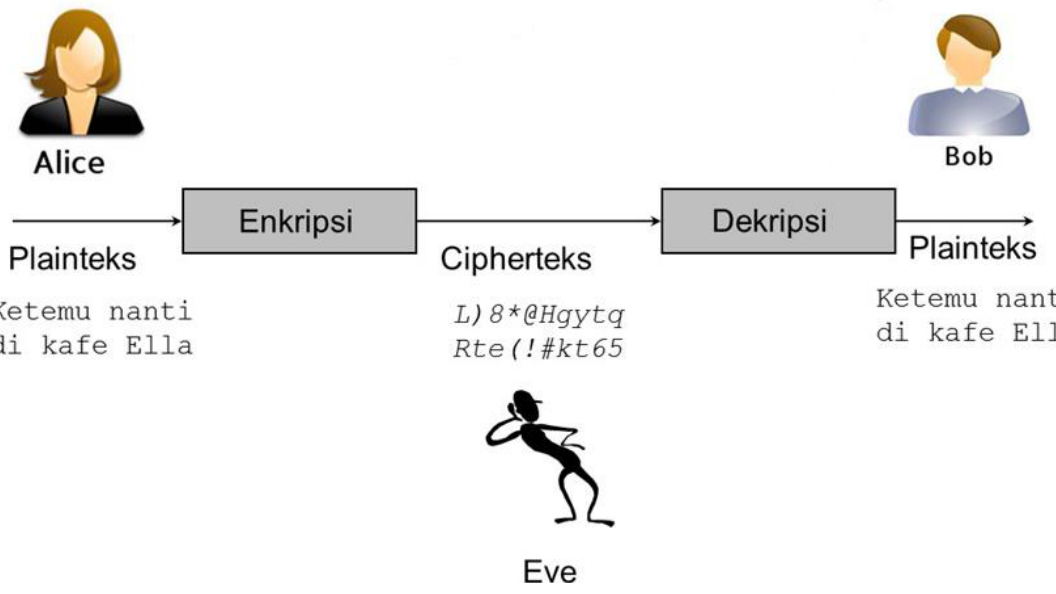
\includegraphics[width=115.50mm,height=163.35mm]{../../images/llm/page_037_img_01.png}%
\end{textblock*}

\end{document}
